\chapter{Лекция}
\label{ch:intro}

\section*{\textbf{Введение}}

На этом занятии вспомним архитектуру цифровой системы связи и рассмотрим BPSK и QPSK модуляции.

\section*{\textbf{Архитектура цифровой системы связи}}

\subsection*{\textbf{Задачи цифровой системы связи}}


Какие задачи у системы связи? Задача системы связи заключается в надежном передать поток бит на заданной скорости по каналу связи. Для передачи по каналу связи мы используем
электромагнитные колебания - sin и cos какой-то частоты.

\subsection*{\textbf{Архитектура передатчика}}


Базовая архитектура цифровой системы связи в простейшем случае состоит из приемника, передатчика и радиоканала. Рассмотрим
упрощенную архитектуру передатчика:

\begin{figure}[H]
    \centering
    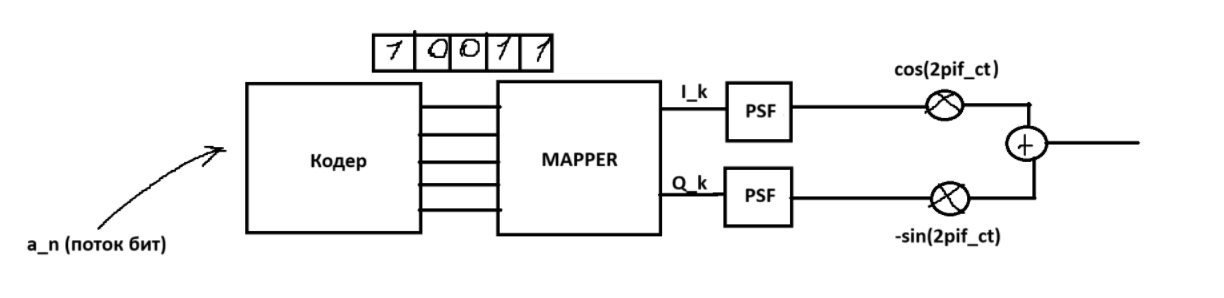
\includegraphics[width=1.0\textwidth]{tx_arch_new.png}
    \caption{Архитектура передатчика}
\end{figure}

Формируется поток бит, который поступает на кодер. В нашем случае кодер просто делит поток бит на блоки определенной длины. У кодера
один вход, по которому последовательно поступают биты, а на выходе N-битная шина, которая уже параллельно передает биты на мапер.
Кодер можно представить в виде схемы следующим образом:

\begin{figure}[H]
    \centering
    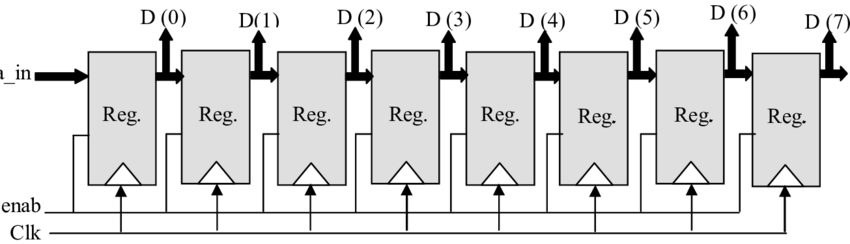
\includegraphics[width=1.0\textwidth]{serial_to_parallel.png}
    \caption{Схема последовательно-параллельного преобразователя}
\end{figure}

Имеется N триггеров с общим тактовым сигналом. По каждому тактовому сигналу поток бит будет "продвигаться" по тригерам и попадать
на N-битную шину, т.е параллельно выводиться из устройства. \\

Далее блоки битов попадают на мапер, который ставит в соответствие каждому блоку числа $I$ и $Q$. Если блок бит имеет размерность N,
то в мапере будет заложено $2^N$ комбинаций. На выходе маппера параллельно получим числа $I$ и $Q$. \\

Сигнал, который мы хоти сформировать имеет вид имеет вид $S_k(t) = I_kcos(2\pi f_ct) - Q_ksin(2\pi f_ct)$, где k - номер текущего символа, 
$I_k$, $Q_k$ - координаты символа в сигнальной диаграмме. Эти координаты мы получаем на выходе маппера. Эти числа в будущем станут парамтерами колебания.

\begin{figure}[H]
    \centering
    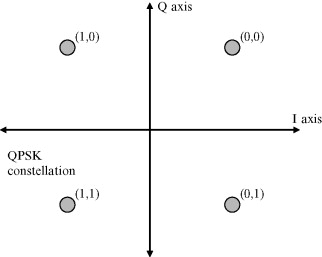
\includegraphics[width=1.0\textwidth]{QPSK.png}
    \caption{Пример сигнальной диаграммы для QPSK модуляции}
\end{figure}

Далее $I$ и $Q$ попадают на Pulse Shaping Filter (PSF). Фильтр выполняет 2 задачи: определяет ширину спектра радиосигнала и его форму, а также применяется
на приемной стороне для символьной синхронизации. Фильтр характеризуется важным параметром во временной области - импульсной характеристикоой $g(t)$.
Импульсная характеристика может быть различной, но для простоты восприятия будем рассматривать только прямоугольную характеристику.
На выходе фильтра получим прямоугольные отрезки сигналов. \\

\begin{figure}[H]
    \centering
    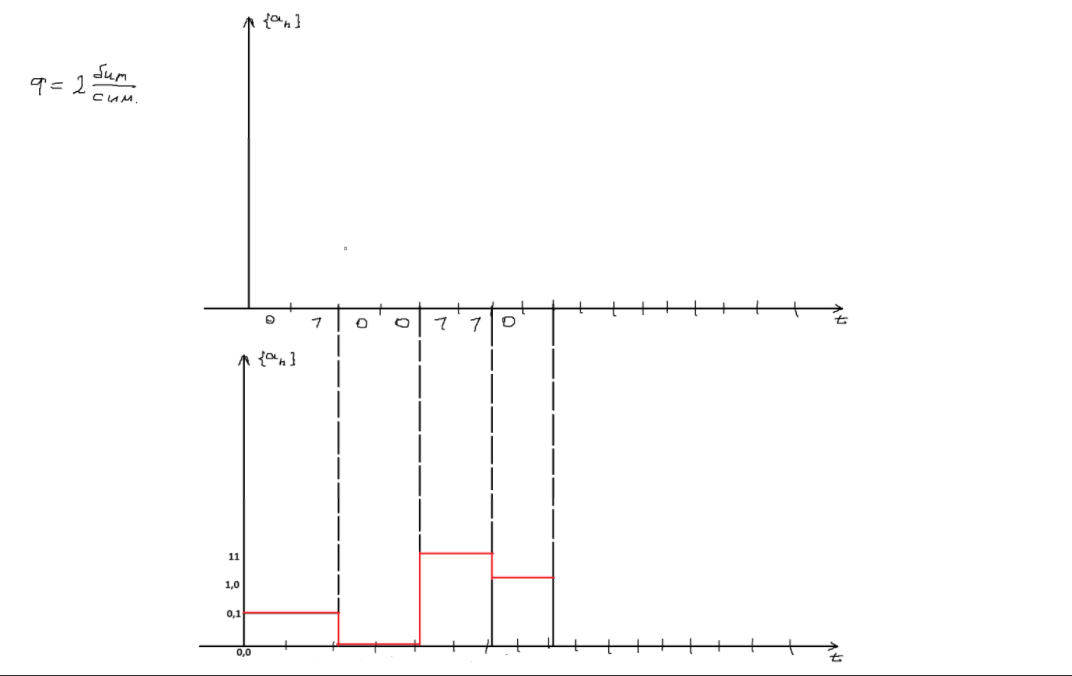
\includegraphics[width=1.0\textwidth]{create_symb.png}
    \caption{Пример формирования символов}
\end{figure}

Длительность символов вычисляется как $1/R_s$, где $R_s$ - символьная скорость. В свою очередь символьная скорость $R_s$ вычисляется
как $R_b/log2(M)$, где $R_b$ - битовая скорость (та скорость, с которой биты поступают на маппер), $M$ - кол-во точек созвездия.
После мапера битовая скорость переходит в символьную, которая определяет длительность прямоугольного импульса.

\section*{\textbf{Схемы модуляции}}

\subsection*{\textbf{BPSK}}

BPSK (Binary Phase Shift Keying) - двухпозиционная фазовая манипуляция. В такой схеме модуляции на 1 бит приходится 1 символ.

\begin{figure}[H]
    \centering
    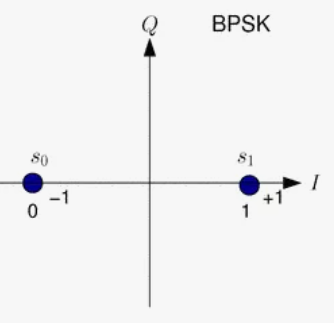
\includegraphics[width=1.0\textwidth]{bpsk.png}
    \caption{Созвездие BPSK модуляции}
\end{figure}

Логика BPSK следующая: если бит имеет сосотяние 0, то он будет соответсвовать сигналу с начальной фазой $\phi$ равной 0, т.е точке
с координатой (1, 0), если бит находится в сосотянии 1, то биту будет соответствовать сигнал с начальной фазой $\phi$ равной $\pi$,т.е 
точке с координатой (-1, 0). Можем заметить, что квадратурная составляющая всегда равна 0, это значит, что в сигнале будет только
cos составляющая, т.к sin составляющая занулится (видно из уравнения сигнала $S_k(t) = I_kcos(2\pi f_ct) - Q_ksin(2\pi f_ct)$).

\begin{figure}[H]
    \centering
    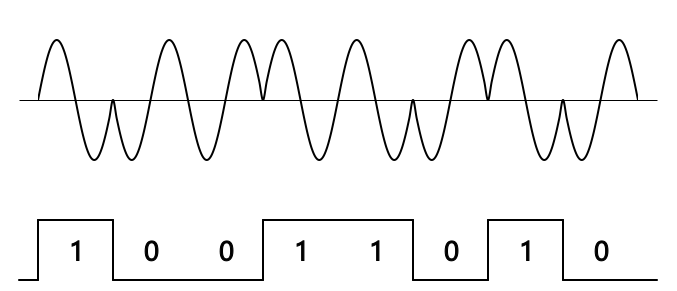
\includegraphics[width=1.0\textwidth]{bpsk_ex.png}
    \caption{Пример кодирования модуляцией BPSK}
\end{figure}

\subsection*{\textbf{QPSK}}

QPSK (Quadrature Phase Shift Keying) - квадратурная фазовая манипуляция. 2 бита кодируются в одном символе. Используется 4 
различных фазы для представления пар битов. Логика этой схемы модуляции такая же, как у BPSK, но уже добавляется квадратурные
составляющие, т.е в сигнале будут как cos составляющая, так и sin составляющая. Точке (0, 0) будет соответсвовать фаза $\frac{\pi}{4}$,
(1, 0) будет соответсвовать фаза $\frac{3\pi}{4}$, (1, 1) будет соответсвовать фаза $\frac{5\pi}{4}$, (0,1) будет соответсвовать фаза $\frac{7\pi}{4}$,

\begin{figure}[H]
    \centering
    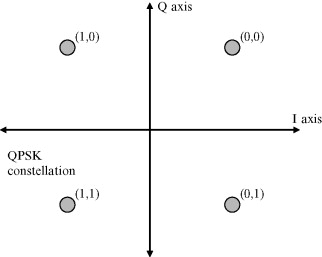
\includegraphics[width=1.0\textwidth]{QPSK.png}
    \caption{QPSK созвездие}
\end{figure}

\begin{figure}[H]
    \centering
    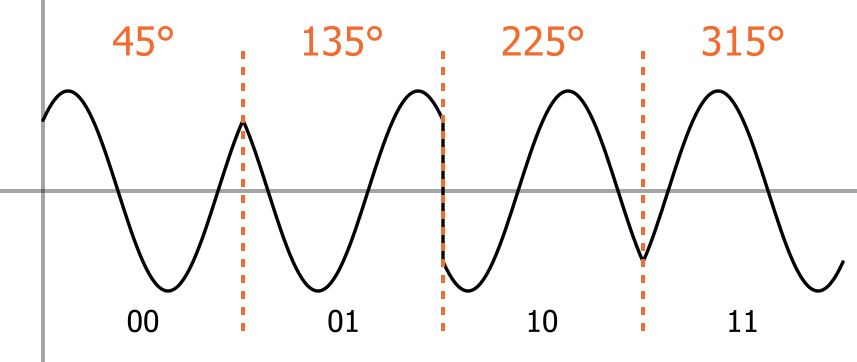
\includegraphics[width=1.0\textwidth]{QPSK_ex.png}
    \caption{Пример кодирования модуляцией QPSK}
\end{figure}


\endinput

